\documentclass[11pt, oneside, a4paper, titlepage]{article}

\usepackage{fancyhdr}
\usepackage{rotating, graphicx}
\usepackage{lscape}
\usepackage{hyperref}
\usepackage{caption}
\usepackage{float}
\usepackage{wrapfig}
\hypersetup{
    colorlinks=true,
    linkcolor=blue,
    filecolor=magenta,      
    urlcolor=cyan,
}

\graphicspath{ {./img/} }

\captionsetup[figure]{labelformat=empty}

\pagestyle{fancy}
\fancyhf{}
\lhead{Assessment Task 3: IT Project}
\lfoot{Team 18 - Creative Protocol\textsuperscript{\textcopyright} 2020}
\rfoot{Page \thepage}

\setcounter{tocdepth}{2}
\setcounter{secnumdepth}{0}

\begin{document}

% Title Page ----
\title{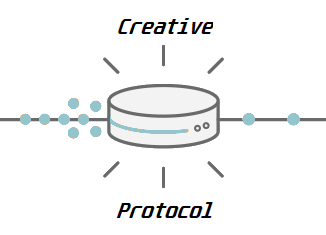
\includegraphics[width=0.7\textwidth]{creative_protocol3}\\
Assessment 3 - IT Project\\
Team Creative Protocol\\
For Introduction to Information Technology (COSC2196)
\\
}

\author{Samuel Ashton, Shane Bunting, Jessica Delgado, William Ericson,\\
 Matthew McCracken, Cameron McLaughlan}

\date{July - August 2020}

\maketitle
% ----


% Blank Page ----
\vspace*{\fill}
\begin{center}
This page intentionally left blank
\end{center}
\vspace*{\fill}
\newpage
% ----


% Table of contents ----
\tableofcontents
\newpage

% Link to websites.
\section{Website Links}
\subsubsection{Group Git Repository}
\paragraph{Assessment 2:}\hfill \break
\url{https://github.com/SamuelPaulAshton/2020SP2Group18A2}
\paragraph{Assessment 3:}\hfill \break
\url{https://github.com/SamuelPaulAshton/2020SP2Group18A3}

\subsubsection{Other Links}
\paragraph{Creative Protocol:}\hfill \break
\url{https://samuelpaulashton.github.io/2020SP2Group18A3/index.html}
\paragraph{Prototype Dashboard:}\hfill \break
\url{https://samuelpaulashton.github.io/2020SP2Group18A3/pages/information.html}

\newpage
% ----


% Personal Information ----
\part{Team Profile}

\section{Contact Details And Profiles}

% Samuel Ashton
\subsection{Samuel Ashton:}
\textbf{Student ID:} \hfill s3742249\\
\textbf{Student email:}\hfill \href{mailto:s3742249@student.rmit.edu.au}{s3742249@student.rmit.edu.au}\\
\textbf{GitHub link:}\hfill \href{https://samuelpaulashton.github.io/IIT/}{https://samuelpaulashton.github.io/IIT/}\\
\\
Hi, I'm Samuel Ashton (s3742249)
\\
\textbf{Team:} Creative Protocol
\\
I am a Brisbane based IT professional, working in the industry for the last 17 years.  Having been interested in IT from an early age I have interacted with technology from the late 80's Starting with an MSX2 microcomputer, watching computing evolve through generations of advancement to today's world of cloud computing and online mobile devices in everyone's pockets.  Throughout my career I have performed roles in IT support, System Administration, Network Engineering and IT Management.  When not in front of a computer, I enjoy fishing with my two children, Japanese sports cars and collecting Phantom comics, even if I don’t get time to read them all! 
\\
\\
\textbf{Ideal Job:} \hfill CTO – Chief Technical Officer - Not Ranked\\
\textbf{Required Skills: }
\begin{itemize}
	\setlength\itemsep{0em}
	\item Communication
	\item	Technical Knowledge of Subject Matter
	\item	Love of Learning
	\item	Adaptability
	\item	Big Picture Thinking
	\item	Diplomacy and Patience
	\item	People Skills
	\item	Strategic Thinking
	\item	Listening
	\item	Coding
	\item	Time Management
	\item	Security and Privacy Management
	\item	Mentoring
\end{itemize}
\newpage

% Shane Bunting
\subsection{Shane Bunting:}
\textbf{Student ID:} \hfill s3407441\\
\textbf{Student email:}\hfill \href{mailto:s3407441@student.rmit.edu.au}{s3407441@student.rmit.edu.au}\\
\textbf{GitHub link:} \hfill \href{https://shanebunting.github.io/IIT/}{https://shanebunting.github.io/IIT/}\\
\\
Hi, I'm Shane Bunting (s3407441)
\\
\textbf{Team:} Creative Protocol 
\\
I am a 27 year old, Melbourne born Libra with my general interests being fitness, cars (Subaru all the way), computers, gaming, animation and security. Straight out of year 12 I went on to complete my certificate 4 in fitness and begin the journey into personal training. It was a weird time for PTs back then and from there I continued to upskill where possible and work on the side where ever I could. I obtained my pre app in electrical, but was unable to land a job due to being of mature age, basically it cost more to hire me.  I also attended university for Game Art and Animation, but financially living expenses where too much at the time, so I had to leave and gain full time employment. Moving forwards, this instead led me to many physical related jobs. This brings us to where I am now, I am on the hunt to pursue my hobbies and turn them into a career in something I am able to commit to long term, as my body has begun to give me signs that it's time to take it back a notch. When I was in year 10, about 15 years old, my parents took my brother and I out of school for a year and we travelled around Australia (Tasmania inc) and also the South island of New Zealand. It was a life changing experience that looking back on wasn’t as bad as 15 year old me made it out to be.
\\
\\
\textbf{Ideal Job:} \hfill Senior Incident Response - Not Ranked\\
\textbf{Required Skills:} 
\begin{itemize}
	\setlength\itemsep{0em}
	\item	Skills probably very closely match Network Security Manager
	\item	Mangement
	\item Communication
	\item Digital Forensics
	\item Cloud Analysis
	\item Reverse Engineering
	\item Penetration, Red Teaming
	\item Threat Hunting
\end{itemize}
\newpage

% Jessica Delgado
\subsection{Jessica Delgado:}
\textbf{Student ID:} \hfill s3864357\\
\textbf{Student email:}\hfill \href{mailto:s3864357@student.rmit.edu.au}{s3864357@student.rmit.edu.au}\\
\textbf{GitHub link:} \hfill \href{https://jessicaprojects.github.io/SP2Demo2020/}{https://jessicaprojects.github.io/SP2Demo2020/} \\
\\
Hi, I'm Jessica Delgado (s3864357) 
\\
\textbf{Team:} Creative Protocol
\\
I am a 28 year old transgender woman living in Sydney and I currently do IT support for eHealth NSW. I am an amateur musician and have learned how to learn play a new instrument every year since age 16. From the age of 18 I completed a Cert IV in Network Administration, Programming and a Diploma of Information Technology. From there I was able to secure employment in a helpdesk role, supporting the largest library of applications used by a single organisation in the southern hemisphere. I have been able to perform various roles within the same organization, moving to application support for the eMR (electronic medical records) systems used in hospitals. I now work as a senior support technician for eHealth. 
\\
\\
\textbf{Ideal Job:} \hfill IT Program Manager - Not Ranked\\
\textbf{Required Skills:} 
\begin{itemize}
	\setlength\itemsep{0em}
	\item Communication
	\item Patience
	\item Technical Skills
	\item Flexibility
	\item Stress Tolerence
	\item Project Management Methodology (Waterfall, Agile, etc)
	\item People and Resource Management
\end{itemize}
\newpage

% William Ericson
\subsection{William Ericson:}
\textbf{Student ID:} \hfill s3866209\\
\textbf{Student email:}\hfill \href{mailto:s3866209@student.rmit.edu.au}{s3866209@student.rmit.edu.au}\\
\textbf{GitHub link:} \hfill \href{https://erics-willi.github.io/ITAssignment1/}{https://erics-willi.github.io/ITAssignment1/}\\
\\
Hi, I'm William Ericson (s3866209) 
\\
\textbf{Team:} Creative Protocol 
\\
For my hobbies, while I enjoy listening to music, I also used to make my own, I studied Music Performance and Technical Production, Yes, I have performed live, no, I will not show you the videos. Over the years, I have hoarded a fair bit of music, while the bulk of my collection is digital (it takes up less space), I also have a sizeable collection of CDs and cassette tapes (and a few records here and there). I've been interested in IT from a young age, it all started when one of my cousins showed me how to use Cheat Engine, while I had fun adding extra stuff to the games I played, I also enjoyed putting in random codes and seeing what it would do. Before joining RMIT, I studied Computing at Deakin College and then Computer Science at Deakin University, but it reached the point where rent was too expensive, so I had to leave.
\\
\\
\textbf{Ideal Job:} \hfill Robotics Engineer - Not Ranked\\
\textbf{Required Skills:} 
\begin{itemize}
	\setlength\itemsep{0em}
	\item Coding
	\item Mathematics
	\item Active Learning
	\item Judgement and Decision Making
	\item Communication
	\item Technology Design
	\item Problem Solving
	\item Persistence
\end{itemize}
\newpage

% Matthew McCracken
\subsection{Matthew McCracken:}
\textbf{Student ID:} \hfill s3864453\\
\textbf{Student email:}\hfill \href{mailto:s3864453@student.rmit.edu.au}{s3864453@student.rmit.edu.au}\\
\textbf{GitHub link:} \hfill \href{https://aussiematt84.github.io/IIT/}{https://aussiematt84.github.io/IIT/}\\
\\
Hi, I'm Matt McCracken (s3864453) 
\\
\textbf{Team:} Creative Protocol 
\\
I am a 35-year-old father of 2, who works full time for a hotel chain where I see to all their IT needs. I was born in Bundaberg, Queensland and, as a young boy, moved to Central West Queensland where I grew up. I currently live in Johannesburg, South Africa. I completed my school career at Barcaldine State School at the end of Grade 11, when I left to pursue a career in IT, as a trainee position opened up at the Department of Main Roads, this is also where I studied my Cert 2 in IT through Tafe. My personal interests are gaming, travel, golf, cricket, and rugby league. I have always had a keen interest in all things tech and like to keep up with what is happening in the world of Technology, both regarding hardware and software. I have always enjoyed understanding how things work, whether it was taking apart an old computer or looking at the source code of how a website was built. My experience in IT include 7 years at The Department of Main Roads following my initial traineeship in their IT department and 6 years as an IT Administrator for a Hotel chain. 
\\
\\
\textbf{Ideal Job:} \hfill OT Network Security Administrator - Not Ranked\\
\textbf{Required Skills: }
\begin{itemize}
	\setlength\itemsep{0em}
	\item CISCO Professional
	\item Problem Solving
	\item Communication
	\item Analytics and Intelligence
\end{itemize}
\newpage

% Cameron McLaughlan
\subsection{Cameron McLaughlan:}
\textbf{Student ID:} \hfill s3717363\\
\textbf{Student email:}\hfill \href{mailto:s3717363@student.rmit.edu.au}{s3717363@student.rmit.edu.au}\\
\textbf{GitHub link:} \hfill \href{https://cammclaughlan.github.io/IT-project-1/}{https://cammclaughlan.github.io/IT-project-1/} \\
\\
Hi, I'm Cameron McLaughlan (s3717363)
\\
\textbf{Team: Creative Protocol}
\\
I am currently 20 years old and working in the Australian army as a rifleman. I currently reside in Townsville but am originally from Melbourne. I completed year 12 in 2017 and have decided that I need to continue my learning and learn about something I am passionate about. My favourite activity to do in my spare time is canoe slalom, which is a field of white-water kayaking. My interest in IT started from a young age I had a relative who worked at apple and always had the newest computers and phones, from that young age I was hooked with all things technology. This love continued as I got into high school and was able to study multimedia in my earlier years, then during my VCE, study software engineering, which is when I realised that I wanted to make some sort of career out of it.  My current career has lead me into signals and radios which has given me a different experience in networking and IP while also exposing me to how many different technologies and systems work and connect together to share data and information around the world securely and undetected. 
\\
\\
\textbf{Ideal Job:} \hfill Software Engineer - Medium Ranked\\
\textbf{Required Skills: }
\begin{itemize}
	\setlength\itemsep{0em}
	\item Coding
	\item Teamwork
	\item Communication
	\item Problem Solving
	\item Multi-tasking
	\item Attention to Detail
\end{itemize}
\newpage
% ----


% Group Processess ----
\section{Group Processess}

\subsection{How did your group work together in Assignment 2? Will you be introducing any changes in process for Assignment 3?}
Based on the group reflection from Assignment 2, although there was a bit of a rocky start, as the group was spread across different tools, once a single collaboration platform was agreed upon things became a lot more smooth. It was found communication was best over Microsoft Teams while collaborating our work using Microsoft OneNote and Office365 worked well for the team and allowed us to work well to complete what needed to be done on the assignment. 

Everybody’s roles in the team was agreed on early, so each member was able to focus on their tasks and keep the team updated on their progress. Regular meetings were also held and minutes were made in the meetings which could be referred back to in subsequent meetings, which allowed group members to stay focused and updated. The minutes also allowed members who may have missed the meeting to stay informed.  

In the beginning phases of the assignment, there was some lack in communication, this was due to various reasons, including location and work commitments. Once communication methods were improved the team worked well together to meet the deadlines.  

We learned that in an online environment, where members have different commitments and schedules, it is of upmost importance that they communicate effectively. It is also vital that each member knows their role and what is expected from them so that deadlines are met or exceeded. 

We thus feel that we have found a formula which works well for our team and we will continue to use this formula going forward in our assignments. 

\subsection{Group Processes and Communications }
Our group is quite diverse in age as well as spread over different time zones, which we initially thought might pose quite a challenge when it came to working as a group and having regular meetings. We found Microsoft Teams best for our meeting which we scheduled for two times a week. We made extensive minutes in the meetings that could be referred back to in the following meetings to see how each member was progressing with their parts of the assignment and to see if anyone needed assistance. The minutes were also helpful in the event that one of the members was unable to attend a meeting due to their schedule or a prior commitment, the minutes would keep them updated as to what had happened in the meeting and the progress of the assignment.  With the use of collaborative tools, we used Microsoft Teams, OneNote and Office365, team members could easily access and share the work done by them in one place so that we were working towards the common goal of completing the task together on time. Backing up our work online was also a great safety measure. Something that we found helpful was that work done by one team member would be read and edited by another team member, leaving us with a document that flowed well.  

\section{Career Plans}
\subsection{Compare and contrast the career plans, including ideal jobs, for each person in the group. What common elements are there, if any? What differentiates each position from the others, if anything? How similar or different are your career plans across the group?}
For each of the ideal jobs chosen by the group, a good foundation is a Bachelor’s Degree in Information Technology as well as obtaining entry level experience in their chosen fields. Although all the ideal jobs start with a Bachelor’s Degree, each one would branch out into their own specific field and specialize in the skills they require for their ideal job. It is also often recommended that an internship be done in the chosen field, this allows for some hands on training as well as being a good opportunity to network which could lead to job offers and also give you good contacts in the IT industry. Another similarity, throughout the IT industry is that anyone in this industry are often expected to keep on top of the latest digital trends, and they should also know how said trends will impact their particular field. 
% ----


% Student Career Plans ----
\section{Career Plans For Ideal Jobs}
\subsubsection{Samuel Ashton - Chief Technical Officer}
A Chief Technical Officer’s primary responsibility is to understand and implement technologies that help a business achieve its goals and objectives. Depending on the size of the organization. Typical Steps to Becoming a Chief Technical Officer are : 
\begin{enumerate}
	\item
    Earn a Bachelor’s Degree. Nearly all Chief Technical Officers start their professional journeys by earning a bachelor’s degree in a computer science-related field. With the knowledge of database design, digital forensics, cyber law, programming, and data integrity, graduates can move on to work in a variety of IT professions.  
    \item
    Aspiring Chief Technical Officers must build a strong educational base and gain experience in entry-level positions before taking the next step toward becoming a Chief Technical Officer. This type of experience can be gained by doing an internship and getting hands on experience in a number of IT areas. 
    \item
    On-the-Job Experience is vital in this position as new problems lead to new IT specialties and roles, the Chief Technical Officer’s job becomes more complex. Organizations depend on their CTOs to have the experience to understand these complexities and to ensure that the right people are in place to address any concerns. CTOs gain this experience and understanding by working in a number of IT areas, such as Network architecture, Big data engineering, Information security management, Security engineering and Web software development. 
    \item
    Positions in the above areas may require only a few years of experience, but professionals need to have between five and 10 years of experience, total, before applying to a manager or director role. Once in a managerial position, an IT manager who wants to work as a CTO must spend an additional five to seven years honing his or her leadership and business skills. So typically a professional must work in the IT field for at least 15 years before seeking employment as a CTO.  
    \item
    After spending some time working in the technology field, IT professionals with the ultimate goal of becoming a CTO should consider pursuing a master’s degree. A CTO needs to have the technological expertise and a keen business sense to be successful in a leadership role.  
\end{enumerate}


\subsection{Shane Bunting - Senior Incident Responder}
Incident responders seek to protect and improve organizational security by preventing, averting, and mitigating security threats. Prevention duties include system monitoring, assessment, testing, and analysis designed to identify and correct potential security breaches. Incident responders often create security plans, policies, protocols, and training that prepare organizations to respond efficiently and effectively to incidents. Steps to become an incident responder : 
\begin{enumerate}
	\item
    Bachelor's or master's degrees in computer forensics, cybersecurity, or a related field often provide ideal educational preparation for incident responders careers. For those seeking a career transition, earning your master's degree in information security or incident response management can position you well for eventually getting upper-level roles such as senior incident responder, senior intrusion analyst, or CSIRT manager. 
	\item
    Many professionals in this skills-based field gain their cybersecurity education simply by earning relevant professional certifications such as certified incident handler, certified intrusion analyst, or certified forensic analyst. Regardless of the degree requirements, most incident responder jobs require some certifications. Keep in mind that certification requirements vary depending on position, employer, and industry. 
	\item
    Someone who wants to become a Senior Incident Responder can benefit from doing an internship, giving them some practical experience in their chosen field and also allowing them to network within the forensic and cybersecurity fields. 
	\item
Most incident responder jobs require at least 2-3 years of prior relevant work experience in fields like computer forensics, cybersecurity, or network administration.
	\item
    Incident responders need considerable applied knowledge and skills working with many kinds of systems. Comprehensive understanding of operating systems, hardware and software systems, and network systems are essential. Related hard skills include system monitoring tools, forensics software, and e-discovery tools. Incident responders also must understand programming languages to do the work often needed to address cybersecurity threats. 
	\item
    Cybersecurity degree programs cultivate skills through coursework in operating systems and information systems security, cybercrime forensics, and object-oriented programming. Aspiring incident responders interested in leadership positions benefit from courses on cybersecurity operations management, cybersecurity law and policy, and global trends. Other relevant courses include cyberwarfare and ethical hacking. 
\end{enumerate}


\subsection{Jessica Delgado - IT Program Manager}
IT project managers oversee and direct the activities of information technology projects, including managing personnel, overseeing budgets and schedules, and executing a project communication plan. Career Steps to Follow to become an IT project manager : 
\begin{enumerate}
	\item
    IT project managers must possess at least a bachelor's degree in computer science, information technology or IT project management. The courses in this program covers topics like Database management systems, IT security, Management information systems, Project procurement management and Principles of project management. 
	\item
    Complete an internship. An internship allows students to interact with experienced IT project managers and complete some of the same tasks they will perform when working in the field. This experience and these networking opportunities may make it easier to find a position in IT project management immediately after graduation. 
	\item
    Most computer and information systems managers have several years of work experience in the field of information technology. Employers often seek candidates who not only possess a bachelor's degree, but who also have experience working in project management or supervising individuals in an information technology department. 
	\item
    After 3-5 years of experience working in an area related to IT project management, many individuals may be able to advance in their careers. IT project managers oversee IT projects by planning the project and managing staff. 
	\item
    To improve employment prospects, consider earning a master's degree.  
	\item
    With enough management experience, IT project managers can advance and become chief technology officers or even chief executives. 
\end{enumerate}
\newpage

\subsection{William Ericson - Robotics Engineer }
Robotics engineers design and build machines to do automated jobs in industries like manufacturing, aerospace and medicine. In order to pursue a career in Robotic Engineering the following steps should be followed : 
\begin{enumerate}
	\item
    Obtaining a Bachelor's degree in IT which offers concentration in robotics as well as Electronics engineering programs that teach you the fundamentals of electronics components and common electronic circuits. Mechanical engineering programs can also be a good qualification as they teach you to apply concepts from physics, mathematics and materials science to create machinery used in transportation, manufacturing, communication and other uses. These programs may also cover electronic, hydraulic and pneumatic systems.  
	\item
    Try to find an internships offered at engineering and robotics companies. An internship can provide you with work experience and help you network within the industry. Your internship might entail no more than observing work or you may be actively involved in a project. 
	\item
    Find a Job as a Robotics Engineer, a good place to start is in the government and technical services sectors. This will allow you to gain work experience and advancement within the robotics engineering field.  
	\item
    You can advance your career and earn a higher salary with a master's degree in robotics engineering. 
\end{enumerate}


\subsection{Matthew McCracken - OT Network Security Administrator}
A Network Security Administrator identifies what type of computer network an organization needs. They install network hardware and software programs, monitor networks, collect data to analyse a network's operation, and train individuals on how to use the network. A good career plan to become a Network Security Administrator is :  
\begin{enumerate}
	\item
    Obtain a Bachelor’s Degree, this is the traditional minimum degree preferred by prospective employers. A Bachelor’s Degree exposes students to a broader curriculum that provides a foundation in mathematics and computer science. Students also develop a comprehensive understanding of programming, software architecture, and software testing. In addition to a Batchelor’s Degree, they can also take specialized courses in application areas, such as Network security, Information technology diagnostics, Network design and Network communications 
	\item
    To improve the chances of getting employment, an internship can be helpful. An internship can allow hands-on experience working with computer networks and also give you the opportunity to network with other professionals in the field. This experience and the networking opportunities may make it easier to find employment after graduation. 
	\item
    Obtain a job and work in the system administrator position to gain the necessary employment in order to work your way up to Network Security Administrator. Security Administrators may backup data contained on an organization's computer network, implement network security measures, monitor network performance, and discuss how to resolve network problems with workers who use the network. 
	\item
    Earning professional certification demonstrates an individual's proficiency in managing specific computer network systems. Many companies prefer certifications, so this will open the door to more job opportunities. Industry companies, such as Cisco and CompTIA, offer certifications to network managers. These certifications, which include the Cisco Certified Network Professional and CompTIA Network+ certification, usually require passing an exam.
	\item
    It is also important to maintain technical skills. The hardware and software programs and computer systems used in network technology and management are constantly changing. Network Security Administrators can remain competitive by staying abreast of the latest technology. 
\end{enumerate}


\subsection{Cameron McLaughlan - Software Engineer }
Software engineering is an ever-changing profession, one that adapts as new technologies are developed. Because of its shifting nature, there are multiple entry points into the profession. A good career plan to become a software engineer is : 
\begin{enumerate}
	\item
    Obtain a Bachelor’s Degree, this is the traditional minimum degree preferred by prospective employers. A Bachelor’s Degree exposes students to a broader curriculum that provides a foundation in mathematics and computer science. Students also develop a comprehensive understanding of programming, software architecture, and software testing. In addition to a Batchelor’s Degree, they can also take specialized courses in application areas, such as networking or embedded systems. 
	\item
    Doing an internship, this can provide students with real world experience. Technology companies may offer internships for students with a bachelor’s who want to expand their skills in specific areas, such as Java, XML or SQL. Internships normally last between three and six months and allow students to work on specific projects or products related to their skills. 
	\item
    Generally speaking, there are two specializations within software engineering: applications and software/systems development. However, distinct areas of practice exist within each of these areas. Software engineers may choose to become experts in a single programming language or type of development. Some examples of speciality areas are Web development, DevOps, Mobile development and Technical stack (e.g., Python, Ruby). 
	\item
    After earning the necessary degree the next step would be to find an entry level job where there are prospects to gain experience.  
	\item
    Software engineering is precise and technical, thus gaining certification verifies an applicant’s knowledge and abilities. Along with experience, certification can improve a person’s marketability. Certifications are available from technology vendors (e.g., Microsoft, Cisco and Oracle) as well as professional organizations (e.g., IEEE) and are tailored to specific areas of practice. 
	\item
    Following up with a Master’s Degree will offer opportunities to qualify for management and leadership positions in the industry.  
\end{enumerate}
\newpage


% ----


% Tools ----
\part{Tools and Technologies}
For our Home Aquaponics Monitoring System (H.A.M.S) there will be two forms of hardware that are required outside the basic laptop/desktop computer which most people have access too. One will be a Raspberry Pi device and the other temperature sensors, which are very cheap and obtainable through many online stores. These two will be the basis for allowing us to create, with further software implementations, a basic set up for monitoring environment variables.  
\\
\\
Alongside the hardware components we will require software and tools such as listed below.  

\begin{itemize}
	\item Raspbian OS
	\item Python
	\item RRDTool
	\item Git
	\item Chart.js Library
	\item Linux Distribution - Debian
	\item SSH Protocol
	\item Nginx
\end{itemize}

All of these tools/resources/software's are open source and readily available to anyone making them ideal for us to use in our product/project without the need for purchasing anything. 

There will be no software licenses needed at present in order to get our H.A.M.S into the initial set up.  

Our group as a whole have had some prior experience in the tools and software listed such as Python, but many of us have not had to deal with software and tools such as RRDTool or Nagios. Through the setup of H.A.M.S, Sam has created, implemented and got the hardware and software set up through the use of a Raspberry Pi device. From this, team members have been able to learn along the way and research topics that we were newly introduced too, expanding our knowledge of devices, software and hardware in relation to our project.  
% ----

% Project Description ----
\part{Project Description}

\section{Project Plan}
\subsection{Overview}
Our project is to build to develop an affordable, scalable aquaponics monitoring and automation solution for back yard hobbyists.  This product will delivered as a cloud platform, known as HAMS (Home Aquaponics Monitoring System), with the long term goal of native mobile to be integrated into the system.  It will involve client devices reporting back to a cloud service, allowing easy monitoring of environment variables and a customisable alerting system 

Large scale automated systems exist for commercial aqua farming but the cost of these solutions make them unviable for the backyard farmer. Conversely, "do it yourself" style projects for monitoring and automating home aquariums also exist, typically using a Raspberry Pi or Arduino board and other consumer electronics to measure different environment factors and present this information on a web-based dashboard. We intend to expand on this idea, targeting environment variables that are core to combining aqua culture and hydroponics, either in a single back yard system or for multiple units on a larger property.  

\subsection{Motivation}
Two of the biggest issues in the world today are food security and climate change. Both these issues are significantly related. As land is cleared for farming, the balance of nature is upset. Crops of plants absorb significantly less carbon dioxide from the atmosphere than the forests that preceded them. Additionally, rainfall is effected by the clearing of forests, resulting in extended droughts in some areas. Traditional plant farming requires lots of water, with additional chemicals used for various reasons, this water tends to run out into local river systems along with trace chemicals causing further issues. 

As our population increases more food is required, further increasing the need for farming and agriculture. Aquaponics is a resource efficient method of growing food, requiring less water than traditional farming, and the symbiotic relationship between the plants and sh results in less chemical additions, such as is the case with separate hydroponics and aquaculture methods. We hope that this project will allow enthusiasts an easy way to understand what is going on with their backyard hobby aquaponics. 

Even if this project does not result in a financially viable product for home aquaponics use, we have specifically chosen to use technologies that are in common use in the IT industry right now. Some are mature, while others relativity new to the IT industry.  This way, as a group we will give ourselves exposure to technology that future employers may be interested in and even use it as a demonstration of our ability .

\subsection{Landscape}
Currently the market for aquaponics monitoring systems has limited solutions for smaller operations, however the market is starting to expand in recent years to accommodate the increased popularity of the agriculture technique. Even more so, aquaponics enthusiasts starting out have limited affordable options available to them. Companies such as Bluelab and GroLine have monitoring systems available, with prices usually being \$500 or more for a basic model with pH and temperature gauges, with limited customizability to the user experience and how data is accessed/stored. Some high end device models have the ability to send your data to a computer or email, however this comes at an increased cost. 

The monitoring system we are suggesting will provide an affordable solution for enthusiasts and small businesses who are wanting to start using aquaponics, with scalability for future expansion. Information is stored in the cloud which is accessible by the user anywhere they have an internet connection via a web browser. The addition cloud technology will allow for expansion into additional features, such as sending a notification of a temperature change to a mobile app. 

\section{Detailed Description}
\begin{wrapfigure}{l}{0.5\textwidth}
	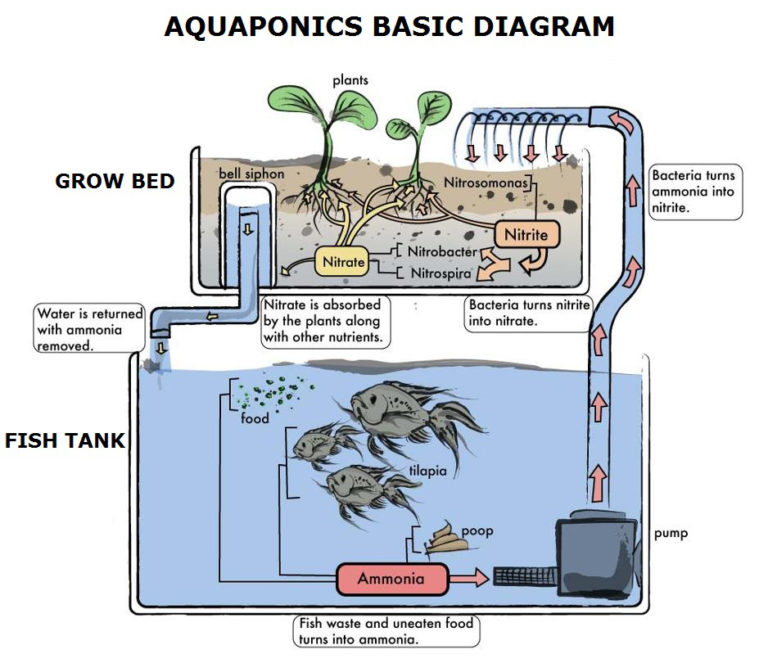
\includegraphics[width=1\linewidth]{DiagramA} 
	\caption{Aquaponics Diagram}
	\label{fig:drawing}
\end{wrapfigure}

For this project, a home-made flood and drain aquaponics system will be used as the 'test subject'. To properly describe the scope of the project, a brief background in Aquaponics is required. Diagram A show the basic concept of how this works.  

\begin{wrapfigure}{r}{0.5\textwidth}
	\includegraphics[width=0.9\linewidth]{DiagramB} 
	\caption{Home Aquaponics Example}
	\label{fig:Aquaponics}
\end{wrapfigure}

Fish are grown in a fish tank, with their waste turning into ammonia as a by-product.  Water is continually being pumped into the grow bed, which is typically above the fish tank, or at least higher. The grow bed is filled with a hydroponics medium such as clay balls, which acts as a biological filter for the fish tank. The ammonia in the water is converted to nitrites and then nitrates as in a typical fish tank filter, but rather than having to regularly change the water to remove the nitrates, the plants within the grow bed absorb them as part of their natural growth.  

The bell siphon ensures that once the water level in the grow bed reaches a pre-determined top level, it siphons the entire grow beds water bac into the fish tank. This ensures that the plants roots are not continually submerged, preventing rot and damage. How often the grow bed is drained is controlled by the flow of water into the grow bed.  

\subsection{Environment Variables}
In order to maintain a healthy aquaponics system and truly understand the science behind it the following environment variables should be monitored and controlled (where possible). 

\subsubsection{Water Temperature}
A consistent water temperature is paramount for the health of sh. Increased growth rates is observed over the warmer months, though too hot a temperature (or too cold) can result in death. 

\subsubsection{Water Levels}
Both Fish and Plants require water to grow, measuring the water levels will not only allow the food and drain cycle to be timed and adjusted accordingly but would also indicate a pumping failure or excess loss of water. 

\subsubsection{PH}
The acidity/alkalinity of the water is also very important to ensure it is in a consistent state, both fish and plants have different PH tolerances depending on the species. Understanding the PH of the water will allow accurate decisions around what plants should be grown. 

\subsubsection{Nitrate/Nitrite}
If an aquaponics systems is working and properly balanced there should be little to no nitrate within the water of the fish tank. If there is, then this would indicate that either the biological filtering of the grow bed is not working or there are not enough plants to absorb the nitrate. Excessive nitrate within the fish tank water is detrimental to fish health and needs to be monitored. Unfortunately this environment variable is one of the most difficult to measure electronically. Some investigation will have to be done to determine whether this measurement is viable. A stop gap solution is to measure this using a chemical test kit and entering the result into the system manually at regular interviews. 

\subsubsection{Sunlight}
Measuring the amount of sunlight the aquaponics system receives will help in analysing growth during the different seasons. 

\section{Aims}
The aim of this project will be to produce multiple client devices that record environment variables at regular intervals and communicate these to a cloud based service, with a web based dashboard to review this information.  We will use Raspberry Pi's as our client devices and IaaS provider such as Amazon Web Service to host cloud the cloud infrastructure required. 

This project can be broken up into several smaller aims, which are listed in approximate order. 

\subsubsection{Concept Pi Client}
Firstly a single stand alone client device will be created, measuring only one variable, water temperature. Temperature sensors are incredibly cheap and easy to obtain to get started and documentation on how to get these working is easy to find.  This will host a local web service simply displaying the temperature history. 

\subsubsection{Concept Dashboard}
A concept dashboard can be developed independently of the pi client.  This will not only allow us to envision what the end product will look like, but serve as a base for the cloud based platform once built.  As RRDTool created graphs are static PNG images generated by RRD Tool itself, we will investigate using an additional library called Chart.js to create real time HTML graphs on our dashboard. 

\subsubsection{Project Documentation and Research}
Throughout the project there is research and documentation required for several reasons.  In order to properly market our project we need to ensure that we are across any other competitive or similar products.  We will also need to completely understand what technical resources and knowledge we require, including possible staff that may be required if this project does get picked up by an investor and turned into more than a proof of concept.  Additionally some technical documentation detailing how the client devices are to be set up and how the system is to be used will need to be created. 

\subsubsection{Initial Concept Pitch}
An initial concept pitch will be created which not only marks the first major milestone in the project, but can also be used to show case what we are intending on developing to potential investors.   This will briefly detail our motivation for starting the project and what we intend to achieve in the short term.  By the time we get to finalising this Initial concept Pitch, we will have a client concept demonstration, pending any unforeseen hurdles we will be able to move forward with developing the cloud based system.  

\subsubsection{Client Sensor Expansion / Client Duplication}
With the original concept raspberry pi completed and tested we will then add further sensors such as water depth, ph, and if financially viable ammonia, and nitrate sensors. Though we do foresee that these will need to be manually entered environment variables into the dashboard for our first release. 

It should now be fairly straight forward to duplicate the client for multiple Aquaponics systems, which can be configured to communicate with the cloud platform later 

\subsection{Cloud Setup}
The cloud setup can be broken down into further tasks, some of which can happen alongside each other. 

\subsubsection{Communications Method}
A secure communications method will need to be implemented or developed to ensure that data between the cloud and the client devices is encrypted.  Environment variables of Aquaponics is not necessarily highly valuable data, but in today's world it is imperative that any Cloud or IoT type device is secured to protect against intrusion.  We could  develop our own client/server based comms method but in the time we have allocated it may be better to use the socket based communications method that RRDtool has built in, but tunnelled over an encrypted SSH connection. 

\subsubsection{Database Structure}
A Simple database structure to store users data such as their login credentials, and their aquaponics systems setups will need to be created for the backend server application to interact with. 

\subsubsection{Server Application}
A backend server application will be written in order to provide an application programming interface (API) to the front end dashboard for retrieval of information for display to the user.  This will take care of database interaction and requesting environment variables in real time from the round robin databases to be fed into the real time graphs on the front end dashboard.  Building the project with a backend application architecture, will ensure easy interoperability with native mobile applications in the future.

\subsubsection{Cloud Deployment}
Actual deployment of both the backend server application and the frontend dashboard to the cloud is a task on its own.  Although IaaS services such as AWS make claims of being able to bring services online within minutes, we will need time to learn the toolset and be comfortable that we have a cloud based solution that not only works but is stable and supportable. 

\subsubsection{Testing}
Testing all parts of the project is paramount to ensure success, hence has been broken up into several sections  See the last page of the report for further details. 

Currently, we have a functioning mock-up client device that is able to log temperature results gathered from a functional aquaponics system, which is then able to be accessed from a developer dashboard. The existing client device and dashboard will be tested and refined to better suit the end user, which will occur over the next two weeks, during which the server team will begin the development of secure communication methods and database structures. Following this testing, there are several weeks which will focus on additional server development and replication of the Pi client device.  

Once the server application has been deployed to the cloud server, multiple Pi clients are then able to be configured to interface with the server application. Once this has been completed we are able to perform full scope testing and further client testing. The desired outcome is that multiple clients are able to log and retrieve their data, with the data reflecting correct temperature results. As the release client device will only feature temperature readings, the initial test group can include local aquariums and aquatic animal owners. 

\subsubsection{Risks}
With the commencement of any project comes the possibility that many things could go wrong, however with the proper risk management processes these risks can be mitigated, with the intention of removing them completely.

Our project includes electronics interfacing with a water source, setting us with the task of ensuring a reliable product while also having a minimalistic design. There are a couple of components that are submerged in water with the potential of 99\% of that components lifespan being spent submerged in water.

As our project will rely on cloud computing a lot of planning will need to go into the implementation of the cloud service. For the initial deployment project we will be looking into IaaS to provide the cloud infrastructure as it would be cost effective and provide more reliability than what could be designed in the outlined timeframe. However the toolsets would need to be learned and understood, with the ability for ongoing support and possible migration to an internally hosted cloud service. It is early in the project to completely mitigate the risks involved in the cloud functionality, however as the project continues to develop it is vital that it is considered in each major step.

A major risk present within our project is a disruption of service. This is a potential risk due to the fact all data is sent to the central server to be processed and logged. If this data is not received by the server, or logged correctly, the end user could face issues with loss of data and potentially having their aquaponics system fail from not receiving a vital notification. To combat this, a custom communications server will be built which will allow for customisable redundancy methods 

\subsection{Final Project Pitch}
Once we have our project finished and tested, we will want another pitch video in order to attract investors.  This will focus more on the cloud based infrastructure and ability to scale the product as a possible subscription based service.  This is where we will propose native mobile apps, which our backend API will already be ready for.  

The chart at the end of the report shows a 16 week project plan, detailing the time frame for each of the above mentioned tasks, note that several of these tasks are dependant of each other and will push forward the time frame if the prior task runs over. 

\subsection{Scope and Limits}
With a limited time frame, the scope of what will be developed as part of this project needs to be defined in order to contain the work required.  Two milestones exist which coincide with the pitch videos.   

The first milestone is at week six of the project. At this stage we will have a single client device measuring temperature and possibly water depth, logging these readings to a round robin database to have graphs generated regularly, and displayed on a single demonstration web site.  We will also have a a concept dashboard for the cloud based login created which will demonstrate the end goal. 

This project will be completed at the end of sixteen weeks, which is the second and final milestone. We will have multiple client devices communicating their data to the cloud service, to be displayed using the dashboard design from the first milestone.  

The use of certain technologies are considered outside the scope of the project and are assumed as existing knowledge.  This includes network connectivity, wireless or otherwise, and administration of IaaS platforms. 

\subsection{Roles}
We will have a product owner who is the main driver of the product, this role is to provide a clear vision and path for the team to develop a successful product. The product owner will be responsible for overseeing the features of the product, while communicating between the stakeholders and project team. 

We will also have a Lead Software Developer that is responsible for overseeing the development and implementation of backend and front end applications. As multiple programming languages and technologies will be utilised, it is important to have someone who is able to integrate the system in the future. One of the main responsibilities of this role is to provide a reliable service that has the ability to expand the organisations technologies.  

To ensure the product is easy to use for the customer, a UI/UX designer will be required. A UI/UX designer has the task of making the users experience as seamless as possible, with the priority on customer satisfaction and continual improvement.  

A Project manager would be required to ensure the project is progressing within the confines of the set timeframe. The project manager is responsible for almost all major phases on a project, managing the budget and scope of the project, and ensuring deadlines are met.  
% ----


% Skills and Jobs ----
\part{Skills and Jobs}
\subsubsection{Front End Web Developer}
A front end web developers skills are focused on building customer facing web applications. They would need to be highly skilled in User Interface design to ensure that the product is intuitive and easy to use. 

Technical skills required would be typical web design languages such as HTML5, PHP and JavaScript. Though we would be probably want to look at getting someone with some experience in a modern web framework such as AngluarJs or Angular. 

We would be looking for a couple of years of experience, working in a team following a consisted development methodology such as Scrum or Agile.  (Note we would probably want to keep the methodology experience consistent across all role candidates)  

\subsubsection{Back End Application Developer}
A Back end developer would work on the actual server side software, including the design of a database to store user information.  They would also look after the communication with the client devices and logging the RRD information on the central server.  They would build an API that the front end developer would utilise in order to retrieve information for display.  They would require previous experience developing REST based API's and have a good understanding of secure web communication protocols 

Technical skills required would be along the lines of: 

Database Design, probably in something like MySQL. (Our project probably wouldn't require the more big data focused database engines such as Mongo or Big Query) 

Server application development, probably in something like nodeJS to go along with a modern web application approach using Angular as a front end. 

\subsubsection{Test Engineer}
In order to ensure that the product is successful, a test engineer will ensure that the product actually works.  They will be able to develop automated test scenarios to ensure that as changes are made they can be tested against standard use cases, giving piece of mind that something else has not been broken somewhere along the line.  They will be able to test the API's built by the back end developer ensuring that they return appropriate results so the Front  end developer can focus on the front end know his/her source data is correct. 

\subsubsection{Dev-Ops Engineer}
A Dev-Ops engineer is role that will definitely be required to ensure that the product is available 24/7.  Any cloud based product requires someone who is responsible for managing software deployments who understands how the product is supposed to work.  They work with both the developers and testers, effectively acting on a provided deployment plan in order to release both new features and bug fixes and are overall responsible for managing the cloud environment. 

We would require someone with experience with cloud environments such as AWS, Microsoft Azure or Google Cloud Platform.  Additionally, in alignment with attempting to ensure that we are using modern technology, they would need experience with managing containers and an orchestration system such as Kubernetes. 
\newpage

\section{Job Advertisements}
\subsubsection{Front End Web Developer}
\textbf{Creative Protocol }
\\
\\
\textbf{About The Role}
\\
Creative Protocol are seeking a web developer with 3 to 5 years' experience in front end web development, who can work well with a team, following a consisted development methodology such as Scrum or Agile. You will be  responsible for implementing visual elements that users see and interact with in a web application, work along side and supported by our back-end web developer, who will be responsible for server-side application logic and integration of the work you produce. We strive to create an amazing user experience so we place a strong emphasis on being able to create a user friendly interface that is like no other. This is an excellent opportunity to be part of a team with a culture of continuous improvement regarding our technologies and practices. 
\\
\\
\textbf{Summary of Responsibilities:}
\begin{itemize}
    	\item Develop usable, accessible, and beautiful user interfaces 
    	\item Build reusable code and libraries for future use. 
    	\item Ensure the technical feasibility of UI/UX designs 
    	\item Optimisation of applications for speed and scalability 
    	\item Manage your workload to meet agreed time frames. 
    	\item Be responsible for gathering and evaluation of all user requirements, illustrating and presenting ideas, producing UI wireframes 
    	\item Proactively bring issues and problems to the attention of the team; generate, propose, and implement innovative solutions to solve them.  solutions to solve them. 
\end{itemize}
\hfill \break
\textbf{About You:}
\begin{itemize}
    	\item A minimum of a bachelor's degree in computer science or equivalent. 
    	\item Possess a keen eye regarding a high level of detail and strive for pixel-perfect design across different web browsers and platforms 
    	\item Expert proficiency with front end web technologies such as HTML / CSS / Javascript 
    	\item A solid understanding of web design, accessibility, usability, search engine optimisation and information architecture 
    	\item PHP / MySQL Back end development 
    	\item Frameworks such as AngluarJs or Angular 
    	\item Understanding of cloud deployments with Docker and AWS 
    	\item Git version control (Github, Bitbucket etc) 
\end{itemize}
\hfill \break
\textbf{What's On Offer?}
\begin{itemize}
    	\item Work in an innovative, design-driven environment. 
    	\item Join a company that values your personal and professional development by providing future growth and development. 
\end{itemize}
\hfill \break
\textbf{How To Apply}
\\
Please submit your resume and cover letter via email to \href{mailto:jobs@creativeprotocol.com.au}{jobs@creativeprotocol.com.au}
\\
\\
Only persons with unlimited rights to work in Australia need apply. 
\\
\\
We are an equal opportunity employer. 
\newpage

\subsubsection{Back End Application Developer}
\textbf{Creative Protocol }
\\
\\
\textbf{About The Role}
\\
Creative Protocol are seeking a Back End Application Developer that has the ability to understand the software development life cycle and leverage a variety of technologies to produce quality software. The role primarily revolves around looking after the communications between the client’s devices and logging the RRD information on the central server. You will also require the ability to to build an API that our Front End Developer can utilise in order to retrieve information for the display. Previous experience in developing REST based API’s with a good understanding of secure web communication protocols will be highly considered. We strive to create an amazing user experience so we place a strong emphasis on our design process. You will be given the opportunity to work with with our team internally and also be responsible for external clients on software design challenges. This is an excellent opportunity to be part of a team with a culture of continuous improvement regarding our technologies and practices. 
\\
\\
\textbf{Summary of Responsibilities:}
\begin{itemize}
	\item Solving problems using logic and methodical testing processes 
	\item Produce high-quality secure code in accordance with our standards
	\item Write and maintain automated tests for code where applicable.
	\item Document code consistently throughout the development process. 
	\item Deliver bug-free code to meet the defined KPIs for software quality and performance. 
	\item Manage your workload to meet agreed time frames. 
	\item Test new programs to ensure that logic and syntax are correct. 
	\item Proactively bring issues and problems to the attention of the team; generate, propose, and implement innovative solutions to solve them. 
\end{itemize}
\hfill \break
\textbf{About You:}
\begin{itemize}
	\item Bachelor’s Degree in Computer Science / IT (Focus on software development) 
    	\item Passionate about all things software and development. 
    	\item Experience in project management, software development, database design and scripting for web applications. 
    	\item Experience and knowledge of Framework such as Angularjs or Angular 
    	\item Experience with SQL databases. 
    	\item Experience with version control tools such as GIT. 
    	\item Experience with other web development frameworks or languages would be a plus (Java, PHP, Python ect) 
    	\item Knowledge of HTML / CSS/ JavaScript. 
\end{itemize}
\hfill \break
\textbf{What's On Offer?}
\begin{itemize}
	\item Work in an innovative, design-driven environment. 
    	\item Join a company that values your personal and professional development by providing future growth and development. 
\end{itemize}
\hfill \break
\textbf{How To Apply}
\\
Please submit your resume and cover letter via email to \href{mailto:jobs@creativeprotocol.com.au}{jobs@creativeprotocol.com.au}
\\
\\
Only persons with unlimited rights to work in Australia need apply. 
\\
\\
We are an equal opportunity employer. 
\newpage

\subsubsection{Test Engineer}
\textbf{Creative Protocol }
\\
\\
\textbf{About The Role}
\\
Creative Protocol are currently looking to aquire a test engineer to work closely in our small team along with software developers and program managers to iron out any bugs in the product, and improve the quality of the finished product. To be successful in this role you will need to to ensure that the product is successful and that our product actually works as intended. You will be required and be able to develop automated test scenarios to ensure that as changes are made they can be tested against standard use cases. This will allow piece of mind that something else has not been broken somewhere along the line. You will be responsible for testing the API's built by the back end developer ensuring that they return appropriate results so the Front end developer can focus on the front end knowing his/her source data is correct. 
\\
\\
\textbf{Summary of Responsibilities:}
\begin{itemize}
    	\item Execution of the agreed project test strategy 
    	\item Taking business and technical requirements and applying a “tester” mindset and skills to build quality through the life cycle 
    	\item Proactive analysis, design and execution of effective test suites within the context of the sprint, includes manual and automation testing 
    	\item Testing front and back end systems using a combination of web services, test harnesses and custom test tools 
    	\item Strong exploratory and scenario testing 
\end{itemize}
\hfill \break
\textbf{About You:}
\begin{itemize}
    	\item 3 to 5 years' experience in test engineering with a good background in development methodology such as Scrum or Agile 

    	\item Ability to identify and capture test cases, trace test results to quality risk; 

    	\item Great analytical Skills 

    	\item Basic understanding of programming concepts 

    	\item Superb time management skills and the ability to stick to deadlines 

    	\item Exposure to Automation and API testing. 

    	\item Good understanding and experience of testing processes, practices and technologies across the entire software life cycle 

    	\item Effective at user story interpretation and converting requirements into relevant and specific test cases 

    	\item Excellent technical, written, and verbal interpersonal communication skills, with a positive attitude and enthusiasm for continuous improvement 
\end{itemize}
\hfill \break
\textbf{What's On Offer?}
\begin{itemize}
	\item Work in an innovative, design-driven environment. 
    	\item Join a company that values your personal and professional development by providing future growth and development.  
\end{itemize}
\hfill \break
\textbf{How To Apply}
\\
Please submit your resume and cover letter via email to \href{mailto:jobs@creativeprotocol.com.au}{jobs@creativeprotocol.com.au}
\\
\\
Only persons with unlimited rights to work in Australia need apply. 
\\
\\
We are an equal opportunity employer. 
\newpage

\subsubsection{Dev-Ops Engineer}
\textbf{Creative Protocol }
\\
\\
\textbf{About The Role}
\\
Creative Protocol are seeking a  a Dev-Ops Engineer to join our small team at Creative Protocol. You will be responsible for ensuring that our product is available 24/7 and have the ability to manage software deployments through great understanding of how the product is supposed to work. You will be working with both our in team developers and testers, acting on a provided deployment plan in order to release both new features as well as bug fixes that may arise. Overall management of our cloud environment will be key in ensuring that our product and services will remain available at all times. This is an excellent opportunity to be part of a team with a culture of continuous improvement regarding our technologies and practices. 
\\
\\
\textbf{Summary of Responsibilities:}
\begin{itemize}
	\item Maintain AWS cloud infrastructure in optimal configuration 
    	\item Ensuring that our product is available 24/7 
    	\item Implement, monitor and improve security configurations using best practice industry and AWS technologies, tools and processes 
    	\item Minimise risk by ensuring knowledge of systems, procedures and processes are documented 
    	\item Manage your workload to meet agreed time frames. 
    	\item Proactively bring issues and problems to the attention of the team; generate, propose, and implement innovative solutions to solve them.
\end{itemize}
\hfill \break
\textbf{About You:}
\begin{itemize}
    	\item A minimum Bacherlor’s degree in computer science with a focus on software development. Equivalent qualifications from industry bodies and vendors may be equally well regarded 
    	\item 3 to 5 years in similar role and any relevant AWS focussed certifications will also be highly regarded. 
    	\item Scripting Skills – JavaScript, Python 
    	\item Multiple OS understanding 
    	\item Good understanding of container management 
    	\item Orchestration System – Kubernetes, Git 
    	\item Experience with Java, Docker, Kafka, SQL 
    	\item Knowledge of web, security, and networking protocols 
    	\item An attitude that favours continuous improvement 
\end{itemize}
\hfill \break
\textbf{What's On Offer?}
\begin{itemize}
	\item Work in an innovative, design-driven environment. 
    	\item Join a company that values your personal and professional development by providing future growth and development.  
\end{itemize}
\hfill \break
\textbf{How To Apply}
\\
Please submit your resume and cover letter via email to \href{mailto:jobs@creativeprotocol.com.au}{jobs@creativeprotocol.com.au}
\\
\\
Only persons with unlimited rights to work in Australia need apply. 
\\
\\
We are an equal opportunity employer. 
\newpage
% ----


% Group Reflection ----
\part{Reflection}
\section{Team Reflection}
\subsubsection{What Went Well:}
Having worked well together on assignment 2 working through assignment 3/5 has been a lot smoother of an experience. We have communicated well over Microsoft Teams while using OneNote for the basis of our assignments. Meetings have been kept to a minimum with everyone knowing what is expected of them, so everyone is able to focus of their tasks and updating OneNote as they progress. With two group assignments due at the same time there was concern this could split up the group and spread our resources too thin, but the group has managed the workload well and managed to complete both assignments on time. 

\subsubsection{What Could Be Improved:}
Having done so well on assignment 2 and with how smoothly assignment 3/5 have gone there hasn't been much space for improvement. That being said having everyone in a similar time zone and with similar work schedules would make attendance at group meetings easier. As these issues that are beyond anyone's control they cannot really be improved upon. 

\subsubsection{What Was Surprising}
As a group we were able to identify one of our major weaknesses for this project, being a lack of communication particularly in the beginning phases. This could be due to time zone differences, current world events, or even prior work commitments. This lapse in communication early on resulted in some of the team feeling the assigning of tasks was delayed resulting in some members having trouble with deadlines. While the team did try to distribute the work evenly, there was some opportunity to share the tasks more evenly throughout the team. By improving communication methods and working towards more collaboration in the team, the above matters would be negligible. 

\subsubsection{What Have You Learnt About Groups:}
Coming to the end of the last of the assignments it was clear to all of us that communicating between one and other and being open about what is happening around the clock really helped get everyone through the assignments as it had done in previous times. The biggest lesson we learnt as a group is that life can and always will get in the way and i think groups has taught us that with appropriate planning  and regular catch ups, that meeting deadlines, be it assignments or not, anything is possible.

\section{Individual Reflection}

\subsection{Samuel Ashton}
\subsubsection{What Went Well:}
I  believe that we went far beyond what was actually required for Assignment 2, so we already had most of the groundwork for Assignment 3 done.  Majority of this assignment was just clarifying details and putting things down to an actual 'project plan' 

\subsubsection{What Could Be Improved:}
Whether it could be improved or not but during this assignment we found that our different circumstances meant that it was almost impossible to meet as a group in entirety.  

\subsubsection{What Was Surprising}
No matter the difference in circumstances, each team member did everything they  could to contribute. Some members had work commitments take them out of communication range, while others were just too busy with work. Even with these hurdles everyone contributed to their best ability. 

\subsubsection{What Have You Learnt About Groups:}
The biggest thing I have learnt about groups during this assignment is to be accepting of others circumstances. Studying remotely is a unique scenario where everyone is at a different stage of life and has different prior commitments. Work 

\subsection{Shane Bunting}
\subsubsection{What Went Well:}
The flow from assignment 2 into assignment 3 was rather easy having completed more than required previously. The other team members stepped up as they did in the last one and tackled a huge portion of the work load. 

\subsubsection{What Could Be Improved:}
Reading the finer details of the assignment itself to pick up little bits and pieces that were missed originally.  

\subsubsection{What Was Surprising}
Just how little there was to add on but also just how much there was to add on from assignment 2. There were a lot of things that stayed the same but took a different angle/approach this time around. 

\subsubsection{What Have You Learnt About Groups:}
That life will always get in the way no matter how much you plan and try and organise. In saying that with the different time zones certain members had, continued work hours and even adventures away things managed to get done as there were people who stepped up and took control of the situations.  

\subsection{Jessica Delgado}
\subsubsection{What Went Well:}
From working with the team on the previous assignment, our previous strengths on communication of set roles early allowed for us to work independently on items and flowing said items into a final project. All communication in our meetings was clear and documented well with meeting minutes being taken and shared for each meeting. There was also continual communication through the use of Microsoft Teams and Discord IM’s, advising team members of changes and upcoming deadlines. Our team was able to communicate openly with members taking on feedback positively. I am quite positive with how my team has been able to work together.

\subsubsection{What Could Be Improved:}
While we had most of the project already defined from the previous assignment, there was often times of doubt with what needed to be done next. We were able to affectively sort out the next steps and coordinate it as a team. A few last minute changes from the team could be better communicated earlier. 

\subsubsection{What Was Surprising}
The most surprising part of working with this team is how we were able to agree on most aspects of the project, the team was able to communicate all feedback productively and all feedback was taken on with considerable thought. Any issues that arose was quickly dealt with which was assisting our team in time management. 

\subsubsection{What Have You Learnt About Groups:}
Real life events will often get in the way of teams being able to communicate or meet up regularly. Often times I have known groups of people to not take real life events into consideration, however this team has been very open and understanding especially considering the current world events and other unforeseen circumstances 

\subsection{William Ericson}
\subsubsection{What Went Well:}
Because we put in a lot of effort in assignment 2, it was easier to do this assignment compared to the previous one. A lot of the groundwork was already done 

\subsubsection{What Could Be Improved:}
It was tough working around peoples schedules, in the final two weeks, it was harder to discuss everything as a complete group. 

\subsubsection{What Was Surprising}
Even though it was tough for everyone's schedule to line up, we managed to get a lot of work done. 

\subsubsection{What Have You Learnt About Groups:}
I learnt to be flexible, not everyone is available when you are and vice versa. 

\subsection{Matthew McCracken}
\subsubsection{What Went Well:}
Having done very well on assignment 2 I feel our group was a lot more ease at the process of the group assignment. I feel there were a lot less unnecessary meetings, most were more comfortable and understood how each member of the group worked. 

\subsubsection{What Could Be Improved:}
Even though I feel the process of the assignment 3/5 was a lot easier then assignment 2 it was still difficult with my time zone being so vastly different to everyone else’s.

\subsubsection{What Was Surprising}
Having seen everyone’s commitment for assignment 2 I was not surprised by all the effort put into assignment 3, it was still great to see everyone working so hard on this assignment.

\subsubsection{What Have You Learnt About Groups:}
Having now completed assignment 2/3/5 as a group I feel a lot easier working with others and having others to rely on in crunch times. That has made look forward to more group tasks in the future.

\subsection{Cameron McLaughlan}
\subsubsection{What Went Well:}
Overall, our group worked very well together. Initially we were spread across different tools before agreeing on a single collaboration platform to work together on.  The use of Microsoft OneNote and Office365 worked extremely well, allowing us to sort and categorise each part of the assignment, and then work together editing others work where necessary.   We agreed on Roles early and each member was able to focus on their tasks, updating the team as they progressed. 

We held regular meetings, documented in meeting minutes which we referred to in each following meeting. This allowed us to ensure that we were focused and had regular status updates.  This also allowed members who may have been unable to attend every meeting a way to stay informed.

\subsubsection{What Could Be Improved:}
As a group we were able to identify one of our major weaknesses for this project, being a lack of communication particularly in the beginning phases. This could be due to time zone differences, current world events, or even prior work commitments. This lapse in communication early on resulted in some of the team feeling the assigning of tasks was delayed resulting in some members having trouble with deadlines.  

While the team did try to distribute the work evenly, there was some opportunity to share the tasks more evenly throughout the team. By improving communication methods and working towards more collaboration in the team, the above matters would be negligible. 

\subsubsection{What Was Surprising}
Some of the things the we found surprising about our group was the diverse backgrounds and age ranges that we all come from, including locations around the world. Even this didn’t affect our ability to collaborate or cooperate.  The group's ability to click and work well from the first meeting were quite surprising adding in everybody's crazy work schedule, it was impressive to see everyone organise themselves around their work and come together to put maximum effort into this assignment. The motivation of everyone in the group over the entire assessment period was impressive and keeping up a tempo like that was surprising.

\subsubsection{What Have You Learnt About Groups:}
The biggest lesson learnt during this group exercise is that communication is key.  In an online environment where members have different commitments and even work in different time zones, communicating availability and progress is paramount.  As a group everyone has learned it is important to make sure work is evenly distributed and that work commitments are known to everyone as so other members can potentially take on a bit more work to keep the team ahead of its own timeline.

\newpage
% ----

\begin{sidewaysfigure}
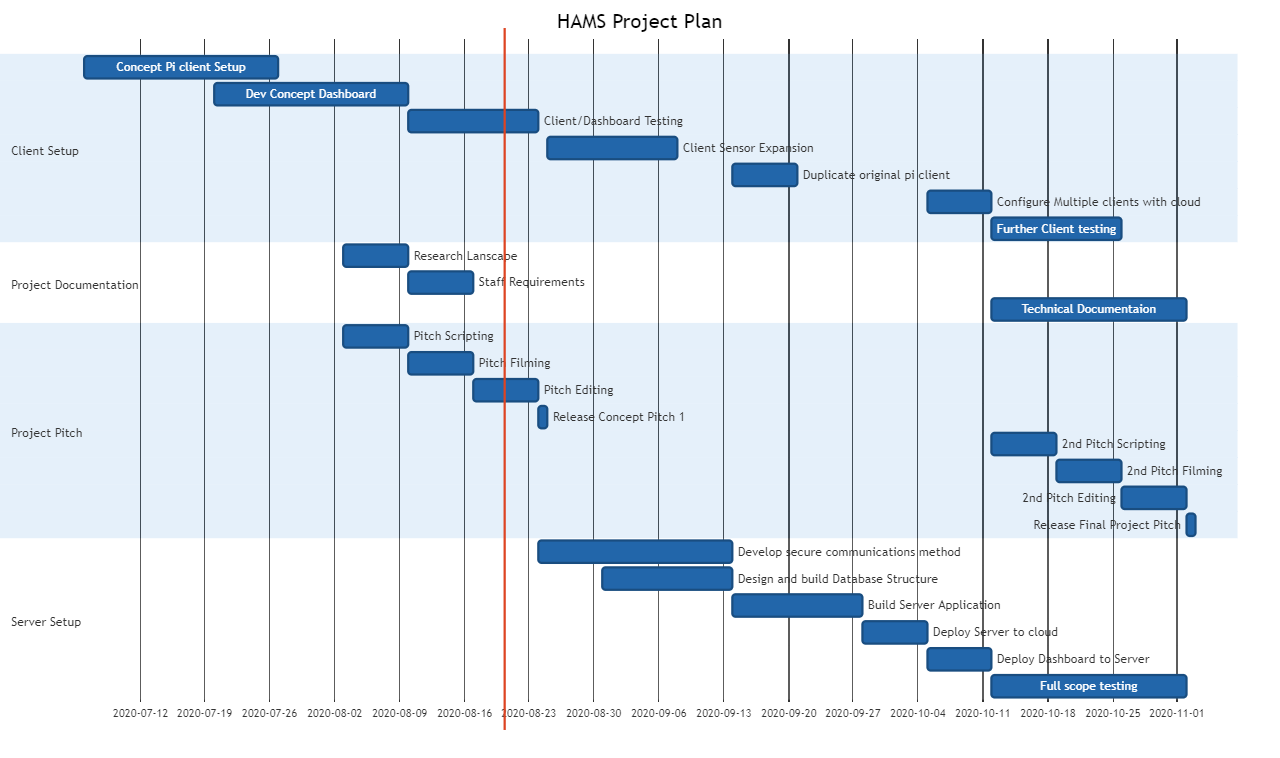
\includegraphics[width=1\textwidth]{DiagramC}
\caption{Gantt Chart for The Project.}
\end{sidewaysfigure}

\end{document}